\documentclass{article}
\usepackage[utf8]{inputenc}
\usepackage[margin=2cm]{geometry}
\usepackage{enumitem}
\usepackage{csquotes}

% maths packages
\usepackage{amsmath}
\usepackage{amssymb}
\usepackage{amsthm}
\usepackage{braket}

% remove space between ket and bra
\renewcommand\bra[1]{{\langle{#1}|}}
\makeatletter
\renewcommand\ket[1]{
  \@ifnextchar\bra{\k@t{#1}\!}{\k@t{#1}}
}
\renewcommand\ket[1]{
  \@ifnextchar\braket{\k@t{#1}\!}{\k@t{#1}}
}
\newcommand\k@t[1]{{|{#1}\rangle}}
\makeatother

% graphics packages
\usepackage{graphicx}
\usepackage{subcaption}
\usepackage[font={small,it}]{caption}
\usepackage{tikz}
\usetikzlibrary{positioning, circuits.logic.US}

% tikz ellipse arcs
\tikzset{
    partial ellipse/.style args={#1:#2:#3}{
        insert path={+ (#1:#3) arc (#1:#2:#3)}
    }
}

\title{Quantum Bernoulli factory}
\author{Suzie Brown \\ {\small supervised by Krzysztof \L atuszy\'nski}}
\date{\today}

% bibliography
\usepackage[round, sort&compress]{natbib}
\usepackage{har2nat} %%% Harvard reference style
\bibliographystyle{agsm}

% theorems
\newtheorem{thm}{Theorem}
\newtheorem{lemma}{Lemma}
\theoremstyle{definition}
\newtheorem{defn}{Definition}
\newtheorem{example}{Example}

% probability symbols
\newcommand{\PR}{\mathbb{P}}
\newcommand{\E}{\mathbb{E}}
\newcommand{\V}{\operatorname{Var}}
\newcommand{\iidsim}{\overset{iid}{\sim}}
\newcommand{\eqdist}{\overset{d}{=}}

% distributions
\newcommand{\Bern}{\operatorname{Bernoulli}}
\newcommand{\Geom}{\operatorname{Geom}}

% project-specific commands
\newcommand{\A}{\mathcal{A}}
\newcommand{\AND}{{\footnotesize AND }}
\newcommand{\NAND}{{\footnotesize NAND }}
\newcommand{\OR}{{\footnotesize OR }}
\newcommand{\NOR}{{\footnotesize NOR }}
\newcommand{\NOT}{{\footnotesize NOT }}

\begin{document}
\maketitle

\section{Introduction}

\section{Quantum information}
From the course by Noah Linden (University of Bristol) and discussion with Thomas Hebdige and David Jennings (Imperial College London). For a comprehensive introduction see for example \citet{nielsen2002} or \citet{wilde2013}.\\

Quantum mechanics is essentially linear algebra in a Hilbert space, with a few additional properties. The definitions in Sections \ref{sec:hilbert_defn} to \ref{sec:linear_ops} are exactly what you would find in a linear algebra course, apart from the notation.

\subsection{Dirac notation}
Dirac notation is a convenient way of denoting vectors such that it is easy to visually identify inner and outer products, and thus quickly recognise scalars, vectors and matrices:

\begin{itemize}
\item $\ket{v}$ denotes a column vector
\item $\bra{v}$ denotes a row vector
\item $\braket{u|v}$ denotes an inner product (resulting in a scalar)
\item $\ket{u}\bra{v}$ denotes an outer product (resulting in a matrix)
\end{itemize}
Additionally, $\overline{\alpha}$ denotes the complex conjugate of a scalar $\alpha$, and $U^\dag$ denotes the adjoint (conjugate transpose) of an operator $U$.

\subsection{Hilbert space}\label{sec:hilbert_defn}
A \emph{Hilbert space} is a vector space with an inner product $\braket{\cdot|\cdot}$ satisfying the following:
\begin{itemize}
\item $\bra{u} (\alpha\ket{v} + \beta\ket{w}) = \alpha\braket{u|v} + \beta\braket{u|w}$
\item $\braket{u|v} = \overline{\braket{v|u}}$
\item $\braket{v|v} \geq 0$ with equality iff $\ket{v}$ is the zero vector.
\end{itemize}

\subsection{Orthonormal bases}\label{sec:onb}
An \emph{orthonormal basis} of a Hilbert space $\mathcal{H}$ is a set of vectors $\{v_1,\dots,v_n\}$ in $\mathcal{H}$ such that:
\begin{itemize}
\item $\operatorname{span}(\{v_1,\dots,v_n\}) = \mathcal{H}$
\item $\braket{v_i|v_j} = \delta_{ij}$
\end{itemize}
Restricting to the space $\mathbb{C}^2$, which is all that is needed to understand the quantum Bernoulli factory, we have the \emph{computational basis} $\{\ket{0}, \ket{1}\} = \{(1,0)^T,(0,1)^T\}$. This is the canonical basis and is henceforth used wherever not specified otherwise. Since it is an orthonormal basis, every vector $\ket{v}$ in $\mathbb{C}^2$ has a unique representation
\begin{equation*}
\ket{v} = \alpha \ket{0} + \beta \ket{1} \equiv (\alpha,\beta)^T
\end{equation*}
for some $\alpha, \beta \in \mathbb{C}$. For reasons which will probably not become apparent in this treatment, we will restrict to \emph{normalised} vectors, requiring also $|\alpha|^2 + |\beta|^2 = 1$.
We will also consider two vectors equivalent if they differ only by an overall phase, i.e.\ $\ket{u} \equiv \ket{v}$ if $\ket{u} = e^{i\theta}\ket{v}$ for some $\theta$. This is because it is impossible to distinguish between two such vectors with any measurement.

To ensure coherency with the properties of the inner product, we have that
\begin{equation*}
\bra{v} = \overline{\alpha} \bra{0} + \overline{\beta} \bra{1}.
\end{equation*}
The inner product of $\ket{u} = u_0\ket{0} + u_1\ket{1}$ with $\ket{v} = v_0\ket{0} + v_1\ket{1}$ is therefore computed as
\begin{align*}
\braket{u|v} &= (\overline{u_0}\bra{0} + \overline{u_1}\bra{1}) (v_0\ket{0} + v_1\ket{1})\\
&= \overline{u_0}v_0\braket{0|0} + \overline{u_0}v_1\braket{0|1} + \overline{u_1}v_0\braket{1|0} + \overline{u_1}v_1\braket{1|1} \\
&= \overline{u_0}v_0 + \overline{u_1}v_1.
\end{align*}
One alternative choice of orthonormal basis which is worth mentioning is given by $\{\ket{+},\ket{-}\}$, consisting of the states
\begin{align*}
&\ket{+} := \frac{1}{\sqrt{2}}(\ket{0} + \ket{1}) \\
&\ket{-} := \frac{1}{\sqrt{2}}(\ket{0} - \ket{1}).
\end{align*}

\subsection{Linear operators}\label{sec:linear_ops}
A linear operator is an operator with the property
\begin{equation*}
A(\alpha\ket{u} + \beta\ket{v}) = \alpha A\ket{u} + \beta A\ket{v}.
\end{equation*}
It is therefore fully defined according to its action on an orthonormal basis. For instance, the quantum \NOT operator (usually denoted $X$) is defined by
\begin{align*}
& X\ket{0} = \ket{1} \\
& X\ket{1} = \ket{0}
\end{align*}
Equivalently, $X$ can be expressed as a matrix with respect to the computational basis:
\begin{equation*}
X = \left(\begin{matrix}
0 & 1 \\ 1 & 0
\end{matrix}\right)
\end{equation*}
In Dirac notation, X can be written in terms of outer products of basis states:
\begin{equation*}
X = \ket{0}\bra{1} + \ket{1}\bra{0}
\end{equation*}
Then if X acts on the state $\ket{v} = \alpha \ket{0} + \beta \ket{1}$, we have
\begin{align*}
X\ket{v} &= (\ket{0}\bra{1} + \ket{1}\bra{0})(\alpha \ket{0} + \beta \ket{1})\\
&= \alpha \ket{0}\braket{1|0} + \alpha \ket{1}\braket{0|0} + \beta \ket{0}\braket{1|1} +
\beta \ket{1}\braket{0|1}\\
&= \alpha \ket{1} + \beta \ket{0}
\end{align*}
as desired.

\begin{itemize}
\item A linear operator $U$ is said to be \emph{self-adjoint} (or \emph{hermitian}) if $U^\dag = U$
\item A linear operator $U$ is said to be \emph{unitary} if $UU^\dag = U^\dag U = I$
\end{itemize}
For example, the operator $X$ is self-adjoint and unitary. Crucially, untiary operators preserve normalisation, so they map states to states. It is also easy to see that unitary transformations are always reversible (i.e.\ the inverse operator exists).

\subsection{Rules of Quantum Mechanics}
\begin{enumerate}
\item \emph{States} of a quantum mechanical system correspond to normalised vectors in Hilbert space, up to an overall phase.
\item \emph{Evolutions} of the system correspond to unitary operators.
\item \emph{Measurements} on quantum states correspond to self-adjoint operators --- see below.
\end{enumerate}

\subsubsection{Spectral theorem and measurement}\label{sec:quantum_mmt}
The outcome of a measurement depends on the state of the system and the type of measurement performed.
The spectral theorem states that every self-adjoint operator $A$ can be represented by its spectral decomposition
\begin{equation}\label{eq:operator_diag}
A = \sum_{i} \lambda_i P_i
\end{equation}
where $\{\lambda_1,\dots, \lambda_k\}$ is the set of \emph{distinct} eigenvalues of $A$, and $P_i$ is the projection operator onto the eigenspace corresponding to eigenvalue $\lambda_i$.

When we measure a state $\ket{x}$ using operator $A$, the measurement outcome we observe is one of the eigenvalues of $A$. In particular, we observe $\lambda_i$ with probability $\bra{x} P_i \ket{x}$.
Making a measurement causes the system to collapse into the eigenstate corresponding to the observed eigenvalue; that is, the state after measurement is proportional to $P_i \ket{x}$.\\

\begin{example}\label{ex:quantum_mmt}
To give a concrete example, let us consider again the operator $X$. This operator has eigenvalues $\pm 1$ corresponding to eigenvectors (known as \emph{eigenstates} in quantum mechanics) $\ket{+}$ and $\ket{-}$ respectively.
Therefore $X$ admits the diagonal representation
\begin{equation*}
X= \ket{+}\bra{+} - \ket{-}\bra{-}
\end{equation*}
which is of the form \eqref{eq:operator_diag}.
Now suppose we make a measurement on the state $\ket{v} = \ket{0}$, using $X$.
The outcome of the measurement will be an eigenvalue of $X$: either $+1$ or $-1$. We observe the outcome $+1$ with probability
\begin{equation*}
\bra{v} P_{+1} \ket{v} = \braket{0|+}\braket{+|0} = 1/2
\end{equation*}
in which case the state after measurement is
\begin{equation*}
P_{+1} \ket{v} = \ket{+} \braket{+|0} \propto \ket{+}.
\end{equation*}
Alternatively, with probability 1/2 we observe the outcome $-1$ and the state after measurement is $\ket{-}$.
\end{example}

In this example, the two outcomes are equally likely because the state is `equidistant' from the two eigenstates of $X$. In general, outcomes that leave the state after measurement closer to the original state are more likely. We will see what is meant by distance between states in Section \ref{sec:bloch_sphere}.

A particularly important type of measurement is measurement in the computational basis. In this case the self-adjoint operator used is $0\cdot \ket{0}\bra{0} +1\cdot \ket{1}\bra{1} = \ket{1}\bra{1}$.
Measuring a state $\ket{v}=\alpha\ket{0} + \beta\ket{1}$ in the computational basis returns 0 with probability $|\alpha|^2$ or 1 with probability $|\beta|^2$. This is particularly useful in quantum computing algorithms because it deterministically converts the basis states $\ket{0}$ and $\ket{1}$ to their classical equivalents 0 and 1, ready for classical output.

\begin{figure}
\centering
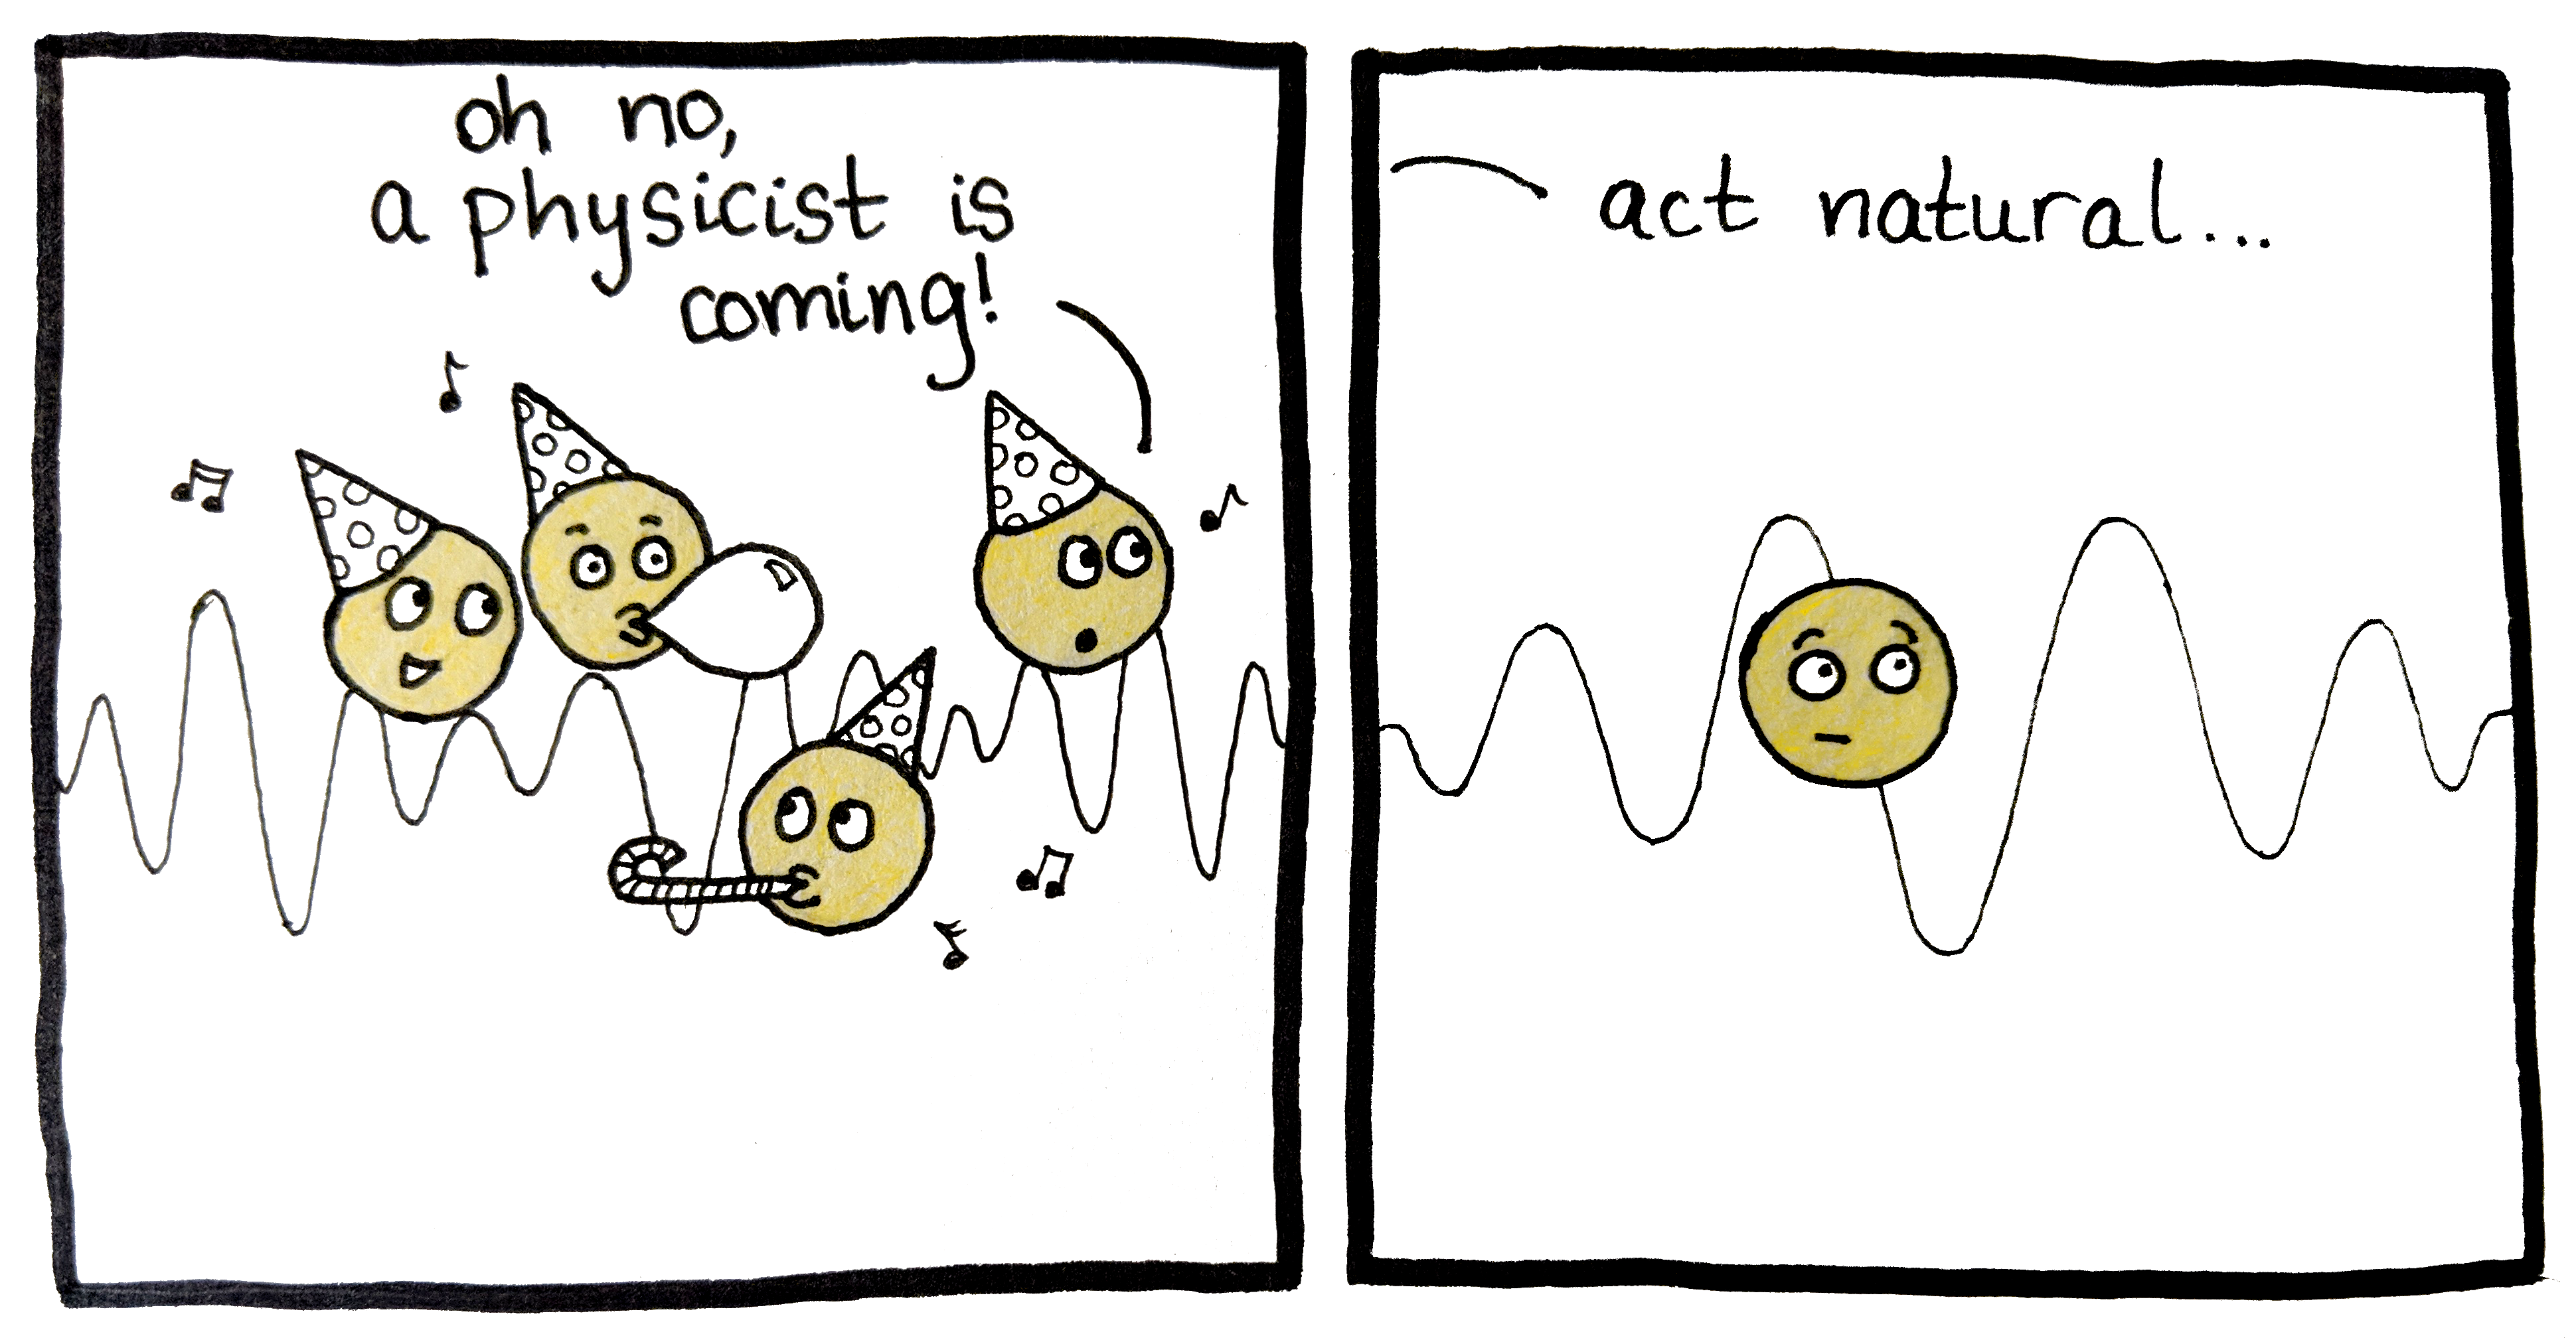
\includegraphics[width=0.8\textwidth]{qit_comic.png}
\caption{When a quantum system is in a superposition of states, making a measurement causes the system to collapse into the eigenstate corresponding to the observed eigenvalue.}
\label{fig:quantum_mmt_comic}
\end{figure}

\subsection{Quantum randomness}
It is worth remarking at this point on the difference between quantum and classical randomness.
As statisticians we are used to dealing with randomness, but we accept that randomness is always part of a model, and is not purported to exist in nature. We artificially introduce random variables into our models to account for a lack of information, either about the state of the system or about the (presumably deterministic) processes that govern certain phenomena.

On the contrary, our uncertainty about the outcome of a measurement on a quantum system is of a different kind. This uncertainty is not a symptom of our lack of knowledge: even when we know exactly the state of the system, as in Example \ref{ex:quantum_mmt}, we are still unable to predict with certainty the outcome of a measurement on the system. The randomness here is intrinsic; it really does exist in nature.

\subsection{Pure and mixed states}
So far we have only encountered \emph{pure states}, like $\ket{0}$ or $\ket{+}$. But we can also consider probabilistic mixtures of pure states, known as \emph{mixed states}, like
\begin{equation*}
\ket{v} = \sum_{i} p_i \ket{v_i}
\end{equation*}
where $\{p_i\}$ is a probability distribution and the $\ket{v_i}$ are pure states.
You can think of this as a `source' which emits a state $\ket{v_i}$ with probability $p_i$.
A classical analogue is a bit which takes the value 1 with probability $p$ or 0 with probability $1-p$ (a $p$-coin). In this case, we can say that the expected value of the bit is $p$.

There is no full ordering on the set of quantum states, so it is not possible to define the expected value of a mixed state. However, we can calculate the expected value of a measurement on a mixed state, using the state's \emph{density operator}.

\subsubsection{Density operators}
The density operator of a mixed state $\ket{v} = \sum_{i} p_i \ket{v_i}$ is given by
\begin{equation*}
\rho = \sum_{i} p_i \ket{v_i}\bra{v_i}.
\end{equation*}
Different mixtures of states may have the same density operator, but in this case is is impossible to distinguish between them by any measurement. For example, a source which emits $\ket{0}$ or $\ket{1}$ each with probability 1/2 has the same density operator $\rho = I/2$ as a source which emits $\ket{+}$ or $\ket{-}$ each with probability 1/2, and the two sources are indistinguishable.

Suppose we measure a mixed state using the self-adjoint operator $A= \sum_k \lambda_k P_k$, where $\{\lambda_k\}$ are the distinct eigenvalues of $A$ and $P_k$ the projection onto the corresponding eigenspace. Recall (from Section \ref{sec:quantum_mmt}) that the outcome of the measurement will be an eigenvalue of $A$. The probability of observing a particular outcome is
\begin{equation*}
\PR(\text{observe }\lambda_j) = \sum_i p_i \bra{v_i} P_j \ket{v_i} = tr(\rho P_j)
\end{equation*}
where $tr(\cdot)$ denotes the trace of an operator.
Note that $tr(\rho)=1$ because the states are normalised and $\{p_i\}$ is a probability distribution.

The state $\rho = I/2$ is called the \emph{maximally mixed} state; it expresses complete ignorance, like a classical (1/2)-coin.

\subsection{The Bloch sphere}\label{sec:bloch_sphere}
Density operators have a neat geometrical representation as points in a unit sphere (Figure \ref{fig:qubit_state_space}). This is called the \emph{Bloch sphere}, and can be thought of as the state space of a quantum bit (qubit).

An arbitrary pure state can be written in the form
\begin{equation*}
\ket{v} = e^{i\psi} \left[ \cos \left(\frac{\theta}{2}\right) \ket{0} + e^{i\phi} \sin \left(\frac{\theta}{2}\right) \ket{1} \right].
\end{equation*}
Since the overall phase $e^{i\psi}$ can be ignored, the state is parametrised by two angles $\theta$ and $\phi$. Taking these as spherical coordinates with unit radius, we can think of each pure state as a point on the unit sphere (or equivalently, a unit vector). Orthogonal states lie opposite each other on the Bloch sphere.
% if theta=0, phi doesn't have any effect...? -use proper coordinates for dens oper

Mixed states can also be represented in the Bloch sphere. The Bloch vector for a mixed state is found by taking the weighted average of the Bloch vectors of its component pure states. Due to the triangle inequality, mixed states therefore lie strictly inside the unit sphere.
This illustrates that several different mixtures of states can have the same density operator. Qubit states are distinguishable if and only if they correspond to different points in the Bloch sphere. %really iff?
%The notion of `distance' between states is formalised as Euclidean distance between points in the Bloch sphere: orthogonal states are the `most different' and lie the furthest possible distance apart on the sphere; while the maximally mixed state is at the centre of the sphere, equidistant from every pure state. %-- not quite right...

There is an analogy here with classical information. The state space of a classical bit is the unit interval: its value could be 0 or 1, or we could take a probabilistic mixture of the two. The `pure' states then are 0 and 1, which lie on the `surface' of the interval, while `mixed' states lie strictly inside the interval (Figure \ref{fig:cbit_state_space}). 


Finally, unitary operators are rotations of the Bloch sphere. This illustrates that unitary transformations are reversible.

\begin{figure}
\centering
\begin{subfigure}{0.25\linewidth}
\centering
\begin{tikzpicture}
\draw (0,4) -- (0,-4);
\filldraw (0,4) circle (2pt) node[anchor=south] {0};
\filldraw (0,-4) circle (2pt) node[anchor=north] {1};
\end{tikzpicture}
\caption{Classical bit}
\label{fig:cbit_state_space}
\end{subfigure}%
\begin{subfigure}{0.75\linewidth}
\centering
\begin{tikzpicture}
\draw (0,0) circle (4cm);
\draw (0,4) -- (0,-4);
\draw[gray] (-4,0) -- (4,0);
\draw[gray] (0,0) ellipse (4cm and 1.5cm);
\filldraw (0,4) circle (2pt) node[anchor=south] {$\ket{0}\bra{0}$};
\filldraw (0,-4) circle (2pt) node[anchor=north] {$\ket{1}\bra{1}$};
\filldraw (-4,0) circle (2pt) node[anchor=east] {$\ket{+}\bra{+}$};
\filldraw (4,0) circle (2pt) node[anchor=west] {$\ket{-}\bra{-}$};
%\filldraw (0,0) circle (2pt) node [anchor=west] {$I/2$};
\draw[ultra thick, ->] (0,0) -- (2,2);
\draw[dotted] (0,0) -- (2,-0.5);
\draw[dotted] (2,-0.5) -- (2,2);
%
\draw[blue] (0,0.5) arc (90:45:0.5);
\draw[red] (0,0) [partial ellipse=180:332:0.5cm and 0.25cm];
\node[red] at (-0.4,-0.4) {$\phi$};
\node[blue] at (0.3, 0.7) {$\theta$};
\end{tikzpicture}
\caption{Qubit}
\label{fig:qubit_state_space}
\end{subfigure}

\caption{State space of classical bits versus qubits. The state space of a classical bit is the line segment $[0,1]$. The `pure' states 0 and 1 are at the endpoints, and probabilistic mixtures of the two lie inbetween. The state space of a qubit is the Bloch sphere. Pure states are on the surface of the sphere, and mixed states lie in the interior. The centre of the sphere is the maximally mixed state $\rho=I/2$.}
\end{figure}

\subsubsection{Geometric view of measurement}
\begin{figure}
\centering
\begin{tikzpicture}
\draw (-5,0) -- (5,0);
\draw (0,-0.1) -- (0,0.1);
\draw (5,0) arc (0:180:5);
\filldraw (-5,0) circle (2pt) node[anchor=east] {$\ket{0}$};
\filldraw (5,0) circle (2pt) node[anchor=west] {$\ket{1}$};
\filldraw (-3,4) circle (2pt) node[anchor=south] {$\ket{v}$};
\draw[->, line width = 1] (-3,4) -- (-3,0);
\draw[dotted] (-3,4) -- (0,0);
\draw[red] (-0.7, 0) arc (180:126:0.7);
\node[red] at (-0.8,0.3) {$\theta$};
\draw[red, <->] (-5,-0.2) -- node[anchor=north] {$x$} (-3,-0.2);
\end{tikzpicture}
\caption{When measuring a state in the computational basis, the probability of observing a certain eigenvalue is related to the projected distance $x$ from the corresponding eigenstate.}
\label{fig:bloch_mmt}
\end{figure}

Suppose we are going to measure a pure state $\ket{v} = \cos \left(\frac{\theta}{2}\right) \ket{0} + e^{i\phi} \sin \left(\frac{\theta}{2}\right) \ket{1}$ in the computational basis. There is a simple relationship between the probability of each outcome and the projection of $\ket{v}$ onto the line segment between $\ket{0}$ and $\ket{1}$ on the Bloch sphere.

Figure \ref{fig:bloch_mmt} shows the semicircular slice of the Bloch sphere on which $\ket{v}$ lies. The value of $\phi$ determines which slice this is, and conditional on that the state only depends on $\theta$ --- the following calculations are independent of $\phi$ and apply to an arbitrary pure state. 
The state $\ket{v}$ is projected onto the line segment between $\ket{0}$ and $\ket{1}$ as shown.
Since the sphere has unit radius, the distance labelled $x$ on Figure \ref{fig:bloch_mmt} is
\begin{equation*}
x = 1-\cos\theta.
\end{equation*}
Using the expansion of $\ket{v}$ in the computational basis, we can calculate the probability of observing measurement outcome 0:
\begin{equation*}
\PR(\text{observe }0) = \braket{v|0}\braket{0|v}
= \cos^2\left(\frac{\theta}{2}\right)
= \frac{\cos\theta + 1}{2}
= 1 - \frac{x}{2}.
\end{equation*}
This relationship between the projected distance and measurement probabilities also applies to mixed states.
If we take any mixture of states with the same value of $\theta$ (but different values of $\phi$), the result will hold, because $x$ and $\PR(\text{observe }0)$ will be the same for every component state, and hence for the mixed state too.
But the result holds for general mixed states as well. Any point in the sphere whose projection onto the line segment between $\ket{0}$ and $\ket{1}$ lies a distance $x$ from $\ket{0}$ will measure 0 with probability $1-x/2$.

Furthermore, this illustrates a more general concept, which applies not only to measurement in the computational basis but to any quantum measurement. 
Any valid measurement operator on one qubit (that is non-trivial in the sense of having more than one possible outcome) has two eigenstates that lie opposite each other on the Bloch sphere. Projecting a state $\ket{v}$ onto the line segment between the two eigenstates gives the probabilities of observing the associated eigenvalues.

\subsection{Entanglement}\label{sec:entanglement}
Suppose we now have two qubits and would like to describe their joint state. 
The joint state space will be $\mathbb{C}^2 \otimes \mathbb{C}^2$, where $\otimes$ denotes the tensor product. This state space has canonical basis
\begin{equation*}
\{ \ket{0}\otimes\ket{0} , \ket{0}\otimes\ket{1} , \ket{1}\otimes\ket{0} , \ket{1}\otimes\ket{1} \}.
\end{equation*}
We also use the shorthand notations $\ket{0}\otimes\ket{0} = \ket{0}\ket{0} = \ket{00}$.
The inner product on $\mathbb{C}^2 \otimes \mathbb{C}^2$ of $\ket{u_1}\ket{u_2}$ with $\ket{v_1}\ket{v_2}$  is defined as $\braket{u_1|v_1}\braket{u_2|v_2}$.

The joint state of two qubits $\ket{u} = \alpha\ket{0} + \beta\ket{1}$ and $\ket{v} = \gamma\ket{0} + \delta\ket{1}$ can be expanded in the computational basis:
\begin{equation*}
\ket{u}\otimes\ket{v} = \alpha\gamma\ket{00} + \alpha\delta\ket{01} + \beta\gamma\ket{10} + \beta\delta\ket{11}.
\end{equation*}
States of this form are called \emph{product states} as they can be written as the tensor product of two states in $\mathbb{C}^2$. However, the set of all product states is only a subset of $\mathbb{C}^2 \otimes \mathbb{C}^2$.
In general, a state $a\ket{00} + b\ket{01} + c\ket{10} + d\ket{11}$ may not be expressible as a product of two states in $\mathbb{C}^2$. In this case, it is called an \emph{entangled} state.

For example, consider the state $(\ket{00} + \ket{11})/\sqrt{2}$. This state is entangled: if we try to write it in the form $\ket{u}\otimes\ket{v}$ as above, we find that either $\alpha$ or $\delta$ must be zero, in which case the coefficient of either $\ket{00}$ or $\ket{11}$ must be zero, producing a contradiction.

The set of entangled states
\begin{equation}
\left\{ \frac{\ket{00}+\ket{11}}{\sqrt{2}} , \frac{\ket{00}-\ket{11}}{\sqrt{2}} , \frac{\ket{01}+\ket{10}}{\sqrt{2}} , \frac{\ket{01}-\ket{10}}{\sqrt{2}} \right\} =: \left\{\ket{\phi^+} , \ket{\phi^-} , \ket{\psi^+} , \ket{\psi^-} \right\}
\end{equation}
is another important basis for $\mathbb{C}^2 \otimes \mathbb{C}^2$, called the \emph{Bell basis}.

\section{Bernoulli factories}
Roughly speaking, a Bernoulli factory is an algorithm that takes samples a $\Bern(p)$ random variable as inputs and uses them to produce a $\Bern(f(p))$ sample as output, where $f$ is a known function but the parameter $p$ is unknown (therefore the algorithm must not depend on $p$).
The imaginary device for generating $\Bern(p)$ random variables is sometimes referred to as a $p$-coin or black box; samples thereof may be called flips/tosses or queries.

%
\begin{defn}[Bernoulli factory]
Let $f: S\to[0,1]$ be a function with domain $S \subseteq [0,1]$, and suppose we have access to a sequence of Bernoulli random variables $X_1,X_2,\dots \iidsim \Bern(p)$ with unknown parameter $p \in [0,1]$. 
Let $U \in \mathcal{U}$ denote a set of auxiliary random variables with known distributions, independent of $p$. Let $\tau$ be a stopping time with respect to the natural filtration, such that $\PR(\tau<\infty)=1$.
\end{defn}
% copy technical defn from some paper...

We follow the terminology of \citet{keane1994}:
\begin{defn}[simulable]
A function $f:S\to[0,1]$ is said to be \emph{simulable} if there is a Bernoulli factory that simulates $f(p)$ for all $p\in S$.
It is \emph{strongly simulable} if there is a Bernoulli factory that simulates $f(p)$ without the need for auxiliary random variables $U$.
\end{defn}

The first formal treatment of a Bernoulli factory problem was presented by \citet{vonneumann1951}, who 
described a Bernoulli factory for the function $f(p)\equiv 1/2$:
\begin{displayquote}
\textit{To cite a human example, for simplicity, in tossing a coin it is probably easier to make two consecutive tosses independent than to toss heads with probability exactly one-half. If independence of successive tosses is assumed, we can reconstruct a 50-50 chance out of even a badly biased coin by tossing twice. If we get heads-heads or tails-tails, we reject the tosses and try again. If we get head-tails (or tails-heads), we accept the result as heads (or tails). The resulting process is rigorously unbiased, although the amended process is at most 25 percent as efficient as ordinary coin-tossing.}
\end{displayquote}

Most authors now use the slightly more convenient convention with the outcomes inverted, so that once 10 or 01 is observed, the output of the Bernoulli factory is equal to the last coin flip (0 or 1 respectively). 
It is clear that, as claimed, this procedure produces a (1/2)-coin, because 01 and 10 appear with the same probability, so conditional on observing one or the other, both outcomes have probability 1/2.
The procedure is formalised in Example \ref{ex:const_half}.

\begin{example}\label{ex:const_half}
$f(p) \equiv 1/2$.\\
This constant function is strongly simulable, using the procedure:
\begin{align*}
& \tau = \min\{ t \in \{2,4,\dots\} : X_{t-1} \neq X_t \} \\
& \A(X_1,X_2,\dots) = X_\tau.
\end{align*}
The running time of this algorithm is random, and indeed unbounded (but it is finite almost surely, making it a valid Bernoulli factory). In particular, $\tau \eqdist 2\times\Geom(2p(1-p))$, with expectation $\E(\tau) = \frac{1}{p(1-p)}$. Figure \ref{fig:runtime_const2} shows the expected running time for various values of $p$. The expected running time achieves its minimum value of four when $p=1/2$ (that is, the coin was already unbiased), hence von Neumann's claim that ``the amended process is at most 25 percent as efficient as ordinary coin-tossing'' (which has deterministic running time one). The expected running time approaches infinity when $p$ is close to 0 or 1, but is moderate across a large range non-extreme values.
\begin{figure}
\centering
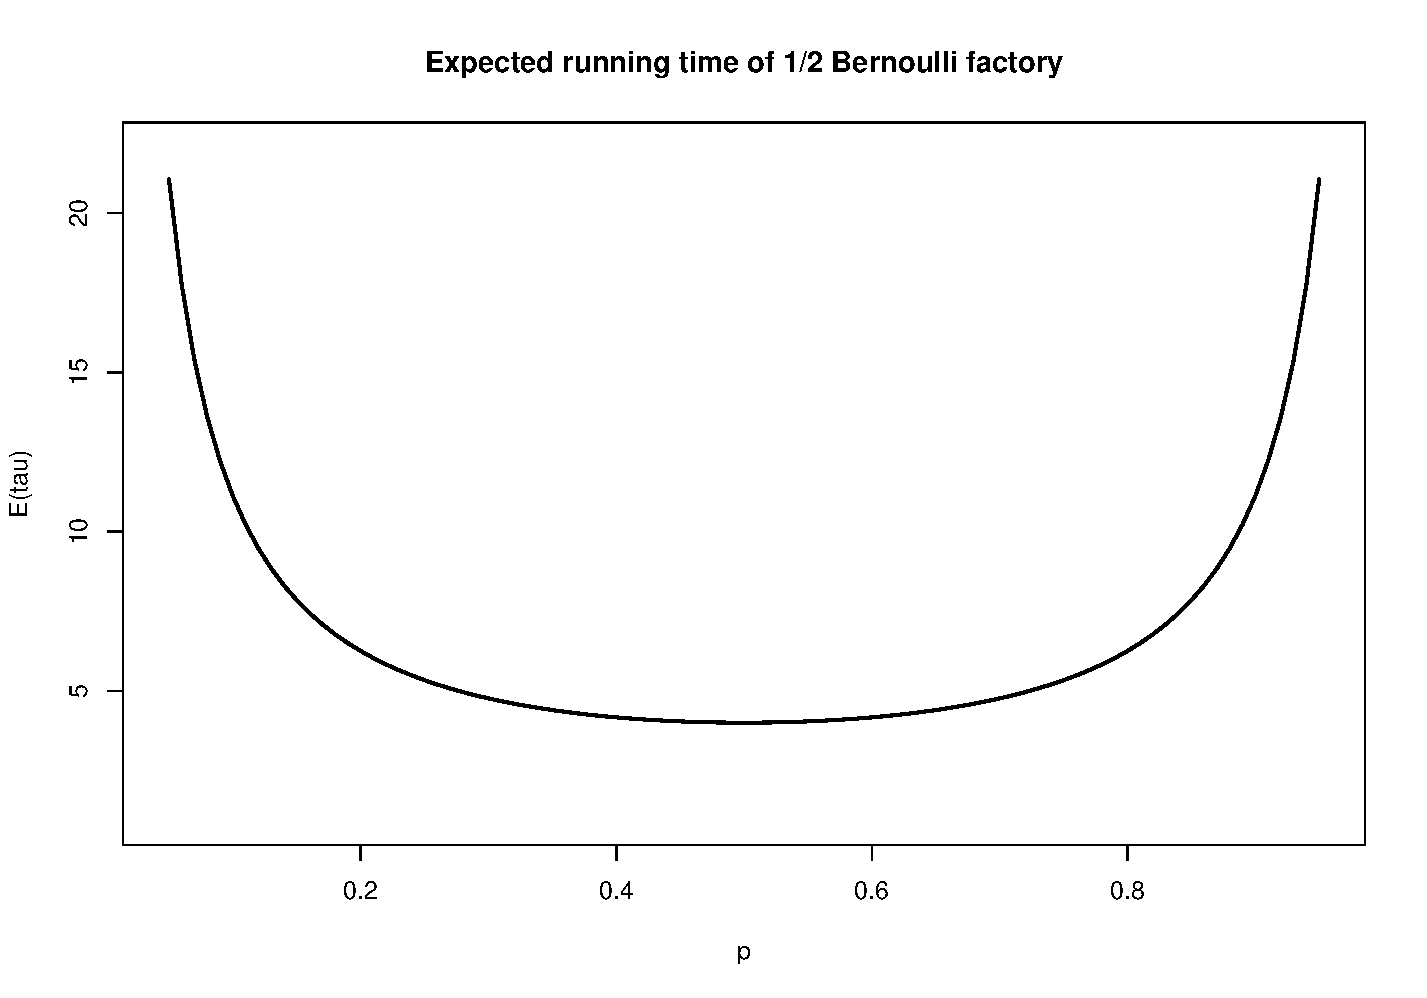
\includegraphics[width=0.8\textwidth]{vonneu_runtime.pdf}
\caption{Expected running time $\E(\tau)$ of von Neumann's Bernoulli factory for $f(p)\equiv 1/2$ \citep{vonneumann1951}.  The expectation attains its minimum $\E(\tau)=4$ at $p=1/2$, and is moderate over a large range of $p$, but grows unboundedly as $p$ approaches 0 and 1.}
\label{fig:runtime_const2}
\end{figure}
\end{example}

The algorithm given in Example \ref{ex:const_half} can be extended to simulate other constant functions of the form $f(p)\equiv 1/k$ for $k\in \{2,3,\dots\}$. The generalised procedure is:
\begin{align*}
& \tau = \min\left\{ t \in \{k,2k,3k,\dots\} : \sum_{i=t-k+1}^t X_{i} = 1 \right\} \\
& \A(X_1,X_2,\dots) = X_\tau.
\end{align*}
However, the running time increases badly with $k$, even under certain early stopping strategies.
Of course, any constant $f(p)\equiv c$ is simulable by employing an auxiliary random variable $U\sim \Bern(c)$, but von Neumann's example shows that $c=1/2$ is also strongly simulable.

Another important example is the case of $f(p)=p^2$, which is strongly simulable using exactly two queries, returning heads if and only if both inputs are heads. Example \ref{ex:bf_pk} presents a generalisation of this procedure.

\begin{example}\label{ex:bf_pk}
$f(p) = p^k, p\in[0,1], k\in\{1,2,\dots\}$.\\
This problem is solved easily by flipping the $p$-coin $k$ times and outputting heads if and only if all $k$ flips return heads. No auxiliary random variable is required.
\begin{align*}
& \tau = k \\
& \A(X_1,\dots,X_T) = \mathbb{I}\{X_1 =1, X_2=1 ,\dots,X_\tau=1\}
\end{align*}
In this case the running time is deterministically equal to $k$. It is clear that this procedure produces heads with probability $p^k$, since the flips are independent and each gives heads with probability $p$.

The running time of this algorithm can be decreased by using an early stopping strategy, whereby we stop the process as soon as a tails input appears (in which case we know immediately that the output will be tails). In this case the running time is random, but still bounded above by $k$:
\begin{equation*}
\tau = k \wedge \min\{t \in \{1,2,\dots\}:X_t=0 \} \eqdist \min\{k, \Geom(1-p)\}.
\end{equation*}
Figure \ref{fig:p2_runtime} shows the expected running time of this procedure for a few values of $k$. We see that early stopping can significantly reduce the expected running time when $p$ is not close to 1, and that the gain in efficiency is greater for larger $k$. In the case $k=1$, where $f$ is the identity, the number of coin flips required is deterministically equal to one, for any $p$.
\begin{figure}
\centering
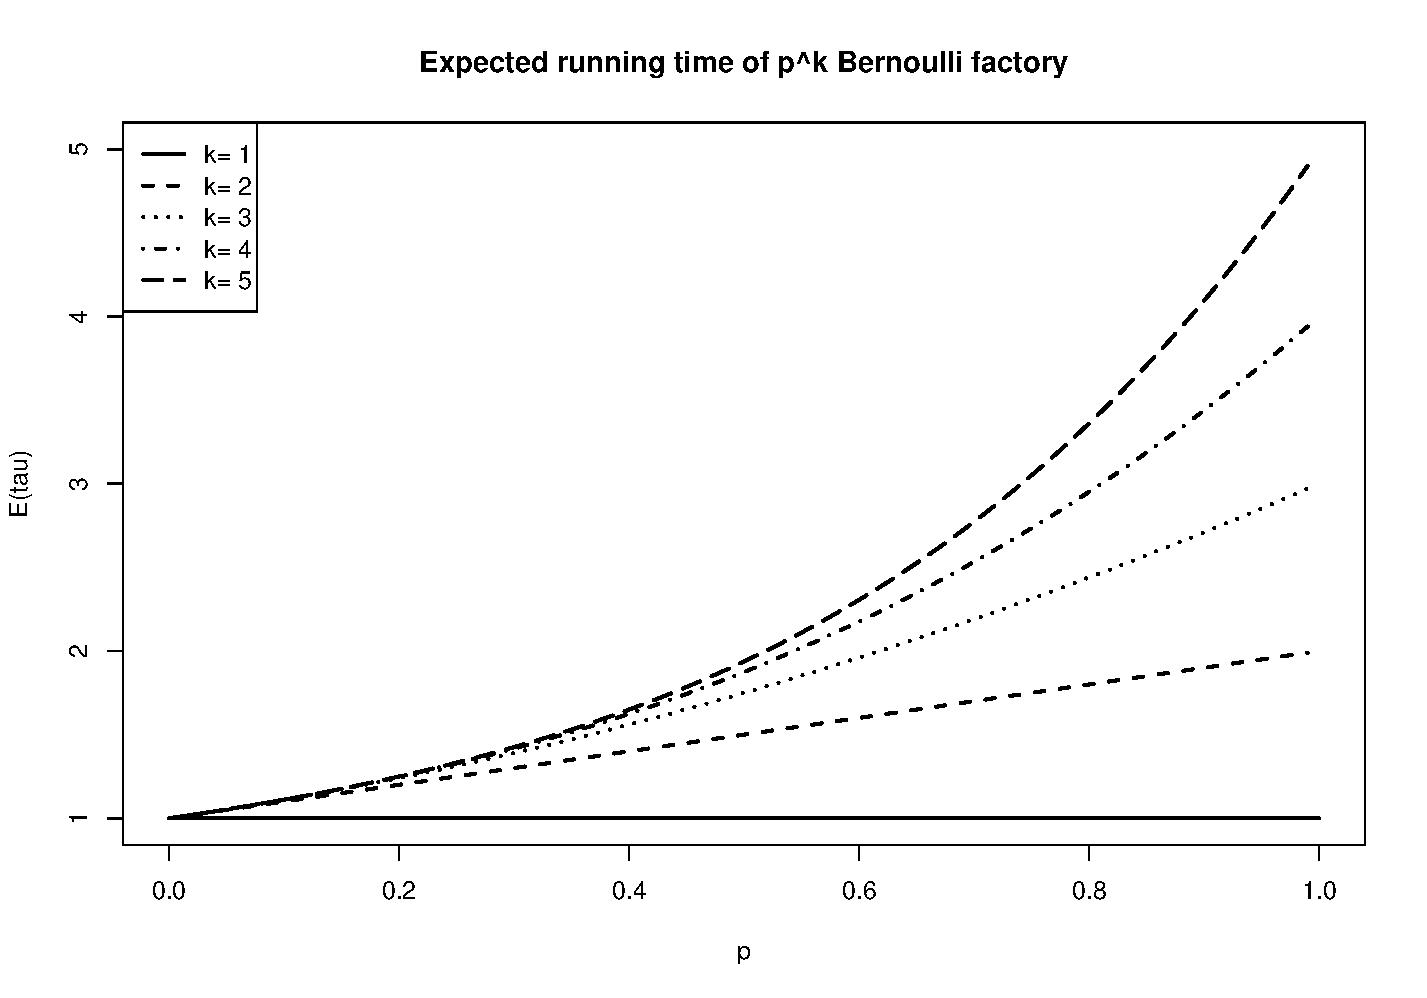
\includegraphics[width=0.8\textwidth]{pk_runtime.pdf}
\caption{Expected running time for the $f(p)=p^k$ Bernoulli factory described, with early stopping. Without early stopping, the running time is deterministically equal to $k$. The early stopping procedure significantly increases the efficiency, particularly when $p$ is small or $k$ is large. The minimum number of queries is one for all $k$ and $p$, and of course the $k=1$ (identity) Bernoulli factory requires exactly one query for any $p$.}\label{fig:p2_runtime}
\end{figure}
\end{example}

% also include example 2p(1-p)

Examples \ref{ex:const_half} and \ref{ex:bf_pk} cast some light on the sort of manipulations that are possible when constructing Bernoulli factories. Lemma \ref{thm:products_compositions} provides some general properties, which are trivial to prove.

\begin{lemma}\label{thm:products_compositions}
Suppose we have a Bernoulli factory $\A_f$ for the function $f:S_f\to[0,1]$ and a Bernoulli factory $\A_g$ for $g:S_g\to R_g\subseteq[0,1]$. Then
\begin{enumerate}[label=(\alph*)]
\item There exists a Bernoulli factory for $1-f: S_f \to [0,1]$, given by inverting the output of $\A_f$.
\item \label{thm:convex_combns} For any $\alpha \in [0,1]$ there exists a Bernoulli factory for $\alpha f + (1-\alpha) g$, given by first sampling from $\Bern(\alpha)$ and, depending on the outcome, using either $f$ or $g$.
\item \label{thm:compositions} If $R_g \subseteq S_f$, then there exists a Bernoulli factory for the composition $f\circ g: S_g \to [0,1]$, given by the composition $\A_f \circ \A_g$.
\item \label{thm:products} There exists a Bernoulli factory for the product $fg:S_f \cap S_g \to [0,1]$, given by $A_f \wedge A_g$.
\end{enumerate}
In the case of \ref{thm:compositions} and \ref{thm:products}, the running time is bounded if and only if the running time of both $A_f$ and $A_g$ is bounded.
\end{lemma}
% might have more properties to add here...

It is not immediately obvious that not all functions are simulable. However, one counterexample is the following.

\begin{example}\label{ex:2p}
$f(p) = 2p, p\in(0,1/2)$.\\
This function turns out not to be simulable, although the truncated function $f(p) = 2p \wedge (1-\varepsilon)$ --- or equivalently, restricting the domain to $p\in(0,(1 - \varepsilon)/2)$ --- is simulable for any $\varepsilon>0$. In this case the number of queries required is $O(\varepsilon ^{-1})$ \citep{huber2016}.

The problem with the unrestricted function is that $f(p)$ approaches 1 within $p\in(0,1)$, which violates one of the necessary and sufficient conditions given in the Keane-O'Brien theorem [REF].
\begin{figure}
\centering
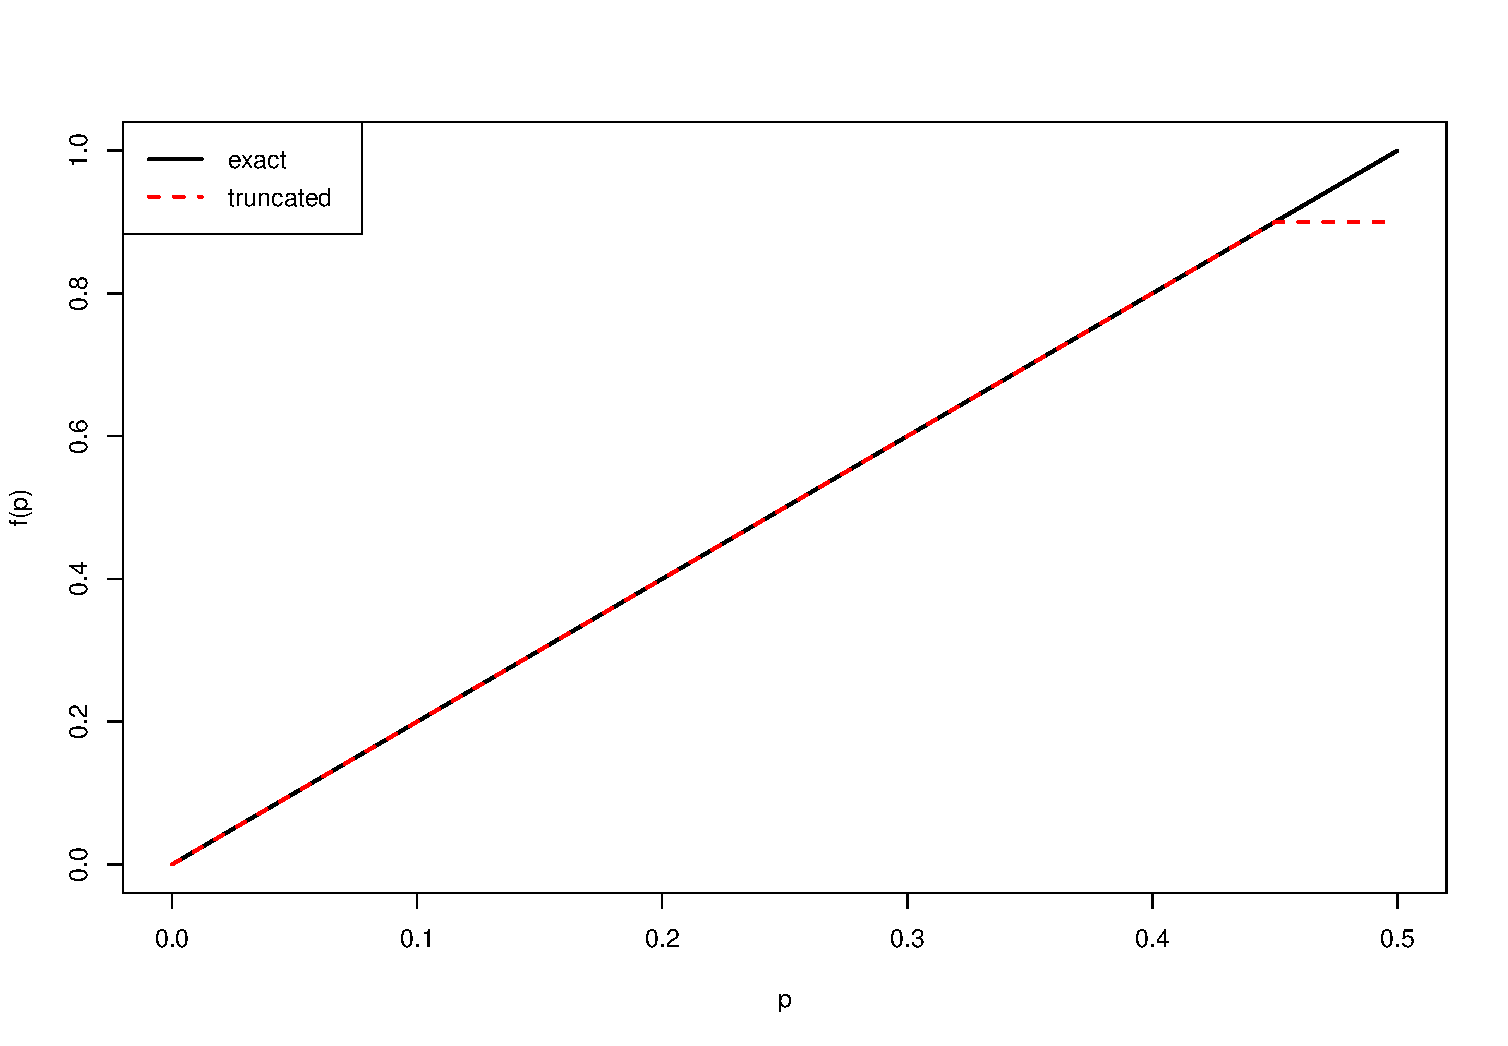
\includegraphics[width=0.8\textwidth]{2p_truncation.pdf}
\caption{The function $f(p)=2p$ (black) is not simulable; whereas the truncated function $f(p)=2p\wedge (1-\varepsilon)$ (red) is simulable for any $\varepsilon>0$, using $O(\varepsilon^{-1})$ queries.}
\label{fig:2p_truncation}
\end{figure}
\end{example}

\begin{thm}
It is not possible to construct a Bernoulli factory for $f(p)=2p$ where $p\in(0,1/2)$.
\end{thm}
The following proof is an intuitive one, adapted from \citet{latuszynski2011}.
The intuition behind the proof is that there is no sharp change between say a (1/4)-coin and a (1/2)-coin; but there is a qualitative difference between the resulting (1/2)-coin and 1-coin respectively. The latter is no longer random, but deterministically returns heads every time, regardless of the outcome on the (1/2)-coin that seeds it.
\begin{proof}
Let $\PR_{p}$ denote the probability measure when the seeding coin has probability $p$ of showing heads. We will compare the cases $p=1/4$ and $p=1/2 - \varepsilon$.
First, 
\begin{equation*}
\lim_{t\to\infty} \PR_{1/4} [\A(X_1,\dots,X_T)=0, T<t] = \frac{1}{2}
\end{equation*}
Thus there exists a $t_0 \in \mathbb{N}$ such that 
\begin{equation*}
\PR_{1/4} [\A(X_1,\dots,X_T)=0, T\leq t_0] > \frac{1}{4}
\end{equation*}
%Now, fixing $\varepsilon>0$, consider the corresponding quantity $\PR_{1/2 - \varepsilon} [\A(X_1,\dots,X_T)=0, T\leq t_0]$; we have the following relation:
We have for any $p \in [1/4, 1/2)$:
\begin{equation*}
\PR_{p} [\A(X_1,\dots,X_T)=0, T\leq t_0] \geq \left(\frac{1}{2}\right)^{t_0} \PR_{1/4} [\A(X_1,\dots,X_T)=0, T\leq t_0] \geq \left(\frac{1}{2}\right)^{t_0+2}
\end{equation*}
Since, restricted to $T\leq t_0$, $\PR_p$ has the same support for any $p \in (0,1)$, we can consider the ratio of probabilities of any sequence in $\{0,1\}^{t_0}$. In particular, we consider 
\begin{equation*}
\inf_{p\in[1/4,1/2)}\, \inf_{A\subseteq\{0,1\}^{t_0}} \frac{\PR_{p}(A)}{\PR_{1/4}(A)}
\end{equation*}
%where the factor of $\left(\frac{1}{2}\right)^{t_0}$ is the largest possible discrepancy between the probabilities of a sequence of $t_0$ flips from a (1/2)-coin or (1/4)-coin.
Now
\begin{equation*}
\PR_{1/2 - \varepsilon} [\text{output } 1] = 1-\PR_{1/2 - \varepsilon} [\A(X_1,X_2,\dots)=0]  \leq 1- \PR_{1/2 - \varepsilon} [\A(X_1,\dots,X_T)=0, T\leq t_0] \leq 1- \left(\frac{1}{2}\right)^{t_0+2}
\end{equation*}
Taking the limit as $\varepsilon\to 0$, the LHS is $f(1/2 - \varepsilon) = 1-2\varepsilon \rightarrow 1$, while the RHS is independent of $\varepsilon$ and remains strictly less than 1. This provides the contradiction, and hence such an algorithm $\A$ cannot exist.
\end{proof}
% not sure if this proof is complete and correct yet...



% present Keane-O'Brien theorem.



\section{The quantum advantage}
It is known that for certain computational problems, quantum computers provide a theoretical advantage over classical computers. For example, the Deutsch-Jozsa algorithm \citep{deutsch1992} is an example of a problem (if not a particularly practical one) which a quantum computer can solve in exponentially less time than the best possible classical algorithm.

It is widely believed (at least within the field) that quantum computing really is more powerful than its classical counterpart. Quantum computers are able to do anything that classical computers can, and quantum speed-ups have been proved for a handful of carefully constructed problems (see for example Grover's algorithm for unstructured search \citep{grover1997}), so from a theoretical viewpoint there is no denying the so-called `quantum supremacy'.

There is, however, a lack of rigorous results for any computational problems with significant practical applications.
One such problem was apparently solved by \citet{kerenidis2016}, who came up with a quantum speed-up for the recommendation problem --- that is, how Amazon and Netflix estimate which products you will like given yours and other customers' ratings of all products. However, the authors were unable to prove that no comparably fast classical algorithm exists, and one has now been found by \citet{tang2018}.

\subsection{A quantum Bernoulli factory}
The Bernoulli factory problem is an example of a practically applicable problem that is nevertheless simple to state and analyse. It was therefore a good candidate for the quest for a practical and provable quantum advantage, and indeed \citet{dale2015} prove this advantage. 

We will use the term \emph{quantum Bernoulli factory} to refer to an algorithm that takes $p$-quoins as inputs, and outputs a $\Bern(f(p))$ sample, where as usual $p\in S$ is unknown and $f:S\to [0,1]$ is known. A $p$-quoin is the quantum analogue of a classical $p$-coin, given by the quantum state
\begin{equation*}
\ket{p} = \sqrt{1-p}\, \ket{0} + \sqrt{p}\, \ket{1}.
\end{equation*}
This is a sensible definition since measuring $\ket{p}$ in the computational basis gives output 0 with probability $1-p$ or 1 with probability $p$, like a classical $p$-coin.
Note that the quantum Bernoulli factory has a quantum input (quoins) and a classical output (measurement outcome).
We will call a function \emph{quantum simulable} if there exists a quantum Bernoulli factory for it.

\citet{dale2015} prove that quantum computation allows a strictly larger class of Bernoulli factories to be constructed, taking as an example the notorious $f(p)=2p$. While this function is not simulable in the classical setting, the authors show that it is quantum simulable, and provide an explicit algorithm using two entangled qubits.
They also determine necessary and sufficient conditions for a function to be quantum simulable, which are weaker than those for classical simulability provided by the Keane-O'Brien theorem [REF].
% with/without entanglement = same set of functions.

Example \ref{ex:qbf_2p} gives the quantum algorithm of \citet{dale2015} for the function $f_\wedge(p) := 2\min\{p, 1-p\}$, $p\in[0,1]$. This function (Figure \ref{fig:wedge_fn}) coincides with that of Example \ref{ex:2p} when the domain is restricted to $p\in(0,1/2)$, so it is clearly sufficient to find a Bernoulli factory for $f_\wedge$.

\begin{figure} % add side-by-side a plot of 4p(1-p) which this problem is boiled down to for the QBF. (or overlay on one plot?)
\centering
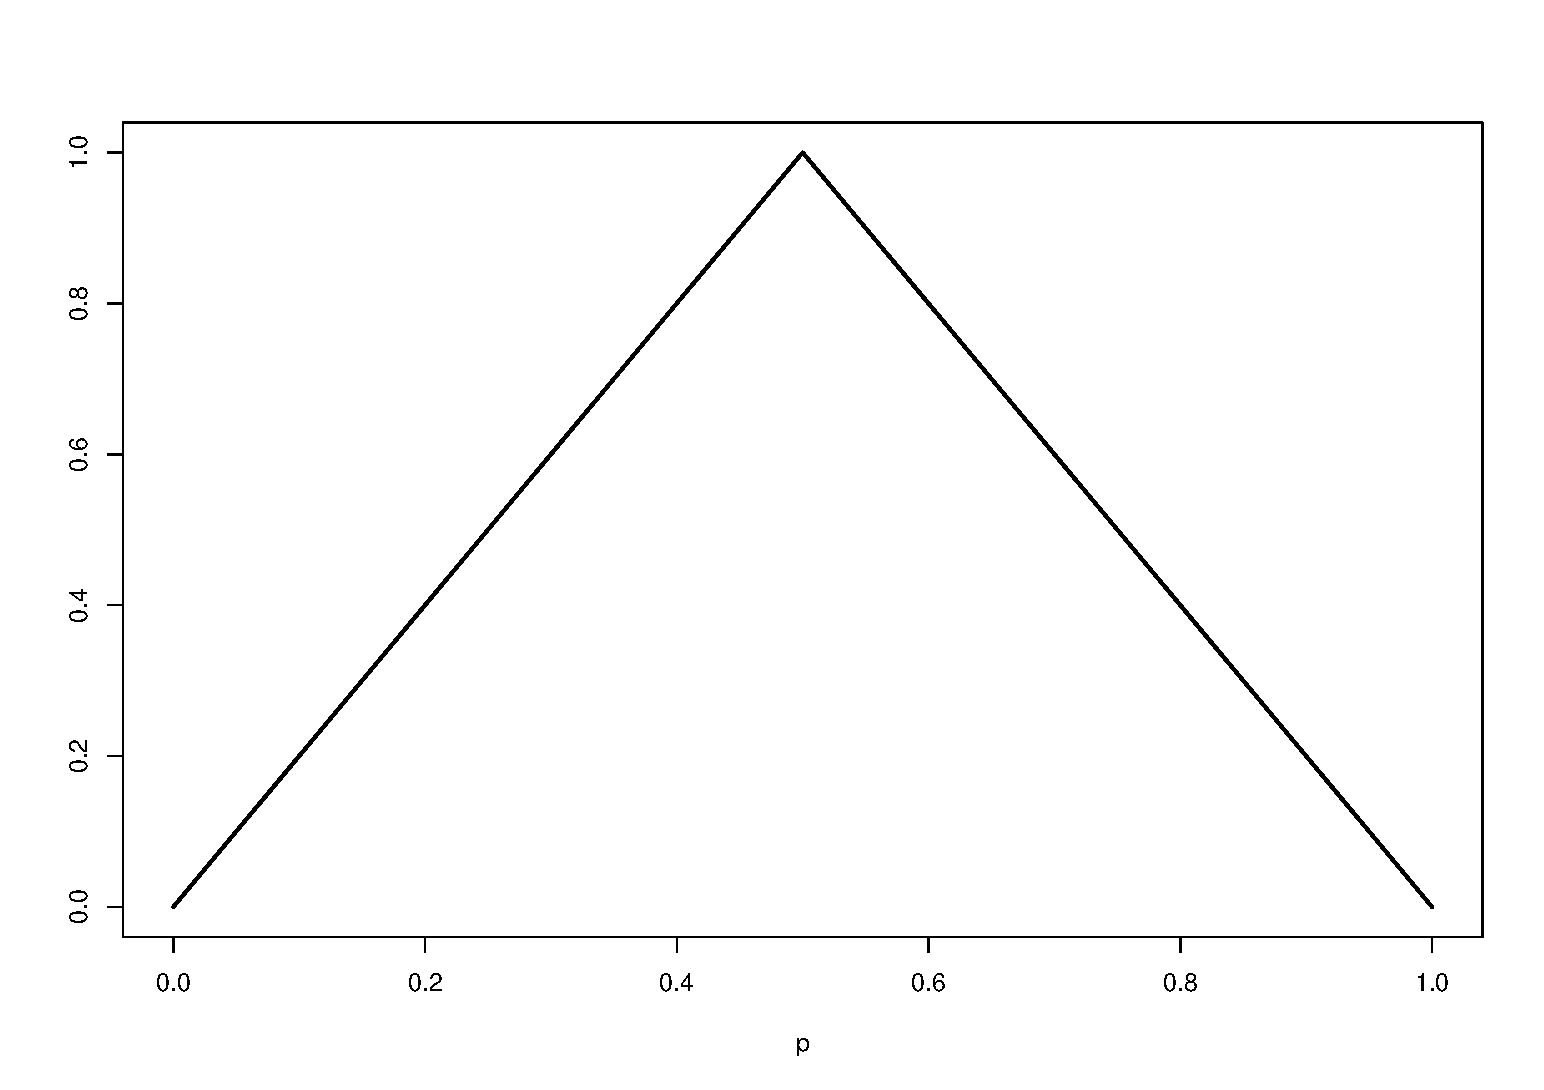
\includegraphics[width=0.8\textwidth]{Wedge_function.pdf}
\caption{•}
\label{fig:wedge_fn}
\end{figure}

\begin{example}\label{ex:qbf_2p}
First note that 
\begin{equation*}
f_\wedge(p) = 2\min\{p, 1-p\} = 1-\sqrt{1-4p(1-p)} = \sum_{k=1}^{\infty} \binom{2k}{k} \frac{1}{(2k-1)2^{2k}} (4p(1-p))^k =: \sum_{k=1}^{\infty} q_k (4p(1-p))^k.
\end{equation*} % check that taylor expansion /!\
where $q_k$ are constants not depending on $p$, and are hence simulable. Due to property \ref{thm:convex_combns} of Lemma \ref{thm:products_compositions}, $f_wedge$ is therefore simulable if there exists a Bernoulli factory for $(4p(1-p))^k$. Since this is a case of Example \ref{ex:bf_pk}, we need only construct a Bernoulli factory for $4p(1-p)$. This function is not classically simulable since it still touches 1 at $p=0.5$.

However, \citet{dale2015} describe the following quantum Bernoulli factory for this function.
We first prepare two quoins; that is, we have two qubits jointly in the product state $\ket{p}\ket{p}$. We then measure the joint state in the Bell basis, say with the operator
\begin{equation*}
0\cdot\ket{\phi^+}\bra{\phi^+} + 1\cdot\ket{\phi^-}\bra{\phi^-} + 2\cdot\ket{\psi^+}\bra{\psi^+} + 3\cdot\ket{\psi^-}\bra{\psi^-}.
\end{equation*} 
Then the measurement outcomes are:
\begin{align*}
&\PR(\text{observe }0) = \braket{v|\phi^+}\braket{\phi^+|v} = 1/2 \\
&\PR(\text{observe }1) = \braket{v|\phi^-}\braket{\phi^-|v} = \frac{(1-2p)^2}{2} \\
&\PR(\text{observe }2) = \braket{v|\psi^+}\braket{\psi^+|v} = 2p(1-p) \\
&\PR(\text{observe }3) = \braket{v|\psi^-}\braket{\psi^-|v} = 0
\end{align*}
This means that $\PR(\text{observe }1 \text{ or } 2) = 1/2$, and $\PR(\text{observe } 2 \mid \text{observe }1 \text{ or } 2) = 4p(1-p)$, which is the required function.
Thus our Bernoulli factory is as follows: measure $\ket{p}\ket{p}$ in the Bell basis until the observed outcome is either 1 or 2, then return heads if the outcome is 2, and tails if the outcome is 1.
\end{example}
% then why does the quoin consumption vary with p???

% CBFs subset of QBFs (Dale eqn 1) ?
% Dale says the classical trucated 2p has poor (exponential) scaling of coin usage with epsilon...?

% present the nec & suf conditions of Dale 2015. cf K-OB thm.

\bibliography{qbf.bib}
\end{document}